% Multivariable Systems Course - Path Following Control Project
% Senior Undergraduate Presentation (25 minutes)

\documentclass[10pt]{beamer}
\usetheme{Madrid}
\usecolortheme{default}

% Packages
\usepackage[utf8]{inputenc}
\usepackage{amsmath}
\usepackage{amssymb}
\usepackage{graphicx}
\usepackage{booktabs}
\usepackage{multirow}
\usepackage{tikz}
\usetikzlibrary{shapes.geometric, arrows, positioning}

% Math commands
\newcommand{\dd}{\mathrm{d}}
\newcommand{\Rset}{\mathbb{R}}

% Title Information
\title[Path Following Control]{Path Following Control for an Ackermann Steering Vehicle}
\subtitle{A Multivariable Control Systems Approach}
\author{Ammar Daher, Baraa Lazkani, Humam Yehia}
\institute{Manara University}
\date{\today}

\begin{document}

% Title Slide
\begin{frame}
  \titlepage
\end{frame}

% Outline
\begin{frame}{Outline}
  \tableofcontents
\end{frame}

% Section 1: Introduction
\section{Introduction}

\begin{frame}{Project Overview}
  \begin{block}{Objective}
    Design and compare multiple control strategies for autonomous path following of an Ackermann steering vehicle
  \end{block}

  \vspace{0.5cm}

  \begin{columns}[c]
    \column{0.5\textwidth}
    \textbf{Controllers Implemented:}
    \begin{itemize}
      \item PID Controller
      \item Stanley Controller
      \item Sliding Mode Controller (SMC)
    \end{itemize}

    \column{0.5\textwidth}
    \textbf{Test Trajectories:}
    \begin{itemize}
      \item Lane Change Maneuver
      \item Circular Path
    \end{itemize}
  \end{columns}

  \vspace{0.5cm}

  \textbf{Implementation:} ROS 2 Jazzy + Gazebo Harmonic Simulation
\end{frame}

\begin{frame}{Why This Project?}
  \begin{itemize}
    \item \textbf{Real-world application}: Autonomous vehicle navigation
    \item \textbf{Multivariable control}: Must control both steering angle $\delta(t)$ and velocity $v(t)$ simultaneously
    \item \textbf{Nonlinear system}: Ackermann kinematics are inherently nonlinear
    \item \textbf{Performance comparison}: Which controller works best for different scenarios?
  \end{itemize}
\end{frame}

% Section 2: Ackermann Steering
\section{Ackermann Steering Vehicle}

\begin{frame}{What is Ackermann Steering?}
  \begin{columns}[c]
    \column{0.5\textwidth}
    \begin{itemize}
      \item Common in cars and most ground vehicles
      \item Front wheels steer, rear wheels fixed
      \item \textbf{Key constraint}: All wheels must roll without slipping
      \item Inner wheel turns at sharper angle than outer wheel
    \end{itemize}

    \column{0.5\textwidth}
    \begin{center}
      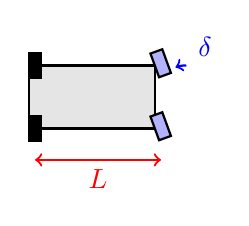
\begin{tikzpicture}[scale=0.8]
        % Vehicle body
        \draw[thick, fill=gray!20] (-1,-0.5) rectangle (1,0.5);

        % Rear wheels (fixed)
        \draw[thick, fill=black] (-1,-0.7) rectangle (-0.8,-0.3);
        \draw[thick, fill=black] (-1,0.3) rectangle (-0.8,0.7);

        % Front wheels (steered)
        \draw[thick, fill=blue!30, rotate around={20:(1,0.5)}] (1,0.3) rectangle (1.2,0.7);
        \draw[thick, fill=blue!30, rotate around={20:(1,-0.5)}] (1,-0.7) rectangle (1.2,-0.3);

        % Wheelbase
        \draw[<->, red, thick] (-0.9,-1) -- (1.1,-1);
        \node[red] at (0.1,-1.3) {$L$};

        % Steering angle
        \draw[->, blue, thick] (1.5,0.5) arc (90:110:0.5);
        \node[blue] at (1.8,0.8) {$\delta$};
      \end{tikzpicture}
    \end{center}
  \end{columns}

  \vspace{0.3cm}

  \begin{block}{Geometric Constraint}
    $$\cot(\delta_o) - \cot(\delta_i) = \frac{w}{L}$$
    where $\delta_o, \delta_i$ are outer and inner wheel angles, $w$ is track width, $L$ is wheelbase
  \end{block}
\end{frame}

\begin{frame}{Kinematic Model}
  \begin{columns}[c]
    \column{0.5\textwidth}
    \textbf{State Variables:}
    \begin{itemize}
      \item Position: $(x, y)$
      \item Heading: $\theta$
      \item Velocity: $v$
    \end{itemize}

    \vspace{0.3cm}

    \textbf{Control Inputs:}
    \begin{itemize}
      \item Steering angle: $\delta$
      \item Velocity command: $v$
    \end{itemize}

    \column{0.5\textwidth}
    \begin{block}{Kinematic Equations}
      \begin{align*}
        \dot{x} &= v \cos(\theta) \\
        \dot{y} &= v \sin(\theta) \\
        \dot{\theta} &= \frac{v}{L} \tan(\delta)
      \end{align*}
    \end{block}
  \end{columns}

  \vspace{0.5cm}

  \begin{alertblock}{Nonlinearity!}
    Note the trigonometric functions ($\cos$, $\sin$, $\tan$) and multiplication of states ($v \cdot \cos(\theta)$). This is a \textbf{nonlinear} system!
  \end{alertblock}
\end{frame}

\begin{frame}{Our Vehicle Parameters}
  \begin{table}
    \centering
    \begin{tabular}{lcc}
      \toprule
      \textbf{Parameter} & \textbf{Symbol} & \textbf{Value} \\
      \midrule
      Wheelbase & $L$ & 0.22 m \\
      Maximum Steering Angle & $\delta_{\max}$ & $\pm 35°$ (0.6109 rad) \\
      Maximum Velocity & $v_{\max}$ & 2.0 m/s \\
      Control Frequency & $f$ & 50 Hz \\
      \bottomrule
    \end{tabular}
  \end{table}

  \vspace{0.3cm}

  \begin{block}{Note}
    This is a \textbf{small-scale} vehicle (22 cm wheelbase), similar to an RC car. The small size makes it highly maneuverable but also sensitive to control parameters.
  \end{block}
\end{frame}

% Section 3: Problem Formulation
\section{Problem Formulation}

\begin{frame}{Path Following Problem}
  \begin{block}{Goal}
    Given a desired path $\mathcal{P} = \{(x_{\text{ref}}(s), y_{\text{ref}}(s), \theta_{\text{ref}}(s))\}$, design a controller to minimize:
  \end{block}

  \begin{itemize}
    \item \textbf{Cross-Track Error (CTE)}: $e(t) = $ perpendicular distance from vehicle to path
    \item \textbf{Heading Error}: $\theta_e(t) = \theta_{\text{ref}} - \theta(t)$
  \end{itemize}

  \vspace{0.3cm}

  \begin{columns}[c]
    \column{0.6\textwidth}
    \begin{block}{Control Objectives}
      \begin{enumerate}
        \item Minimize CTE: $|e(t)| \to 0$
        \item Align heading: $|\theta_e(t)| \to 0$
        \item Smooth control: avoid aggressive steering
        \item Track velocity profile
      \end{enumerate}
    \end{block}

    \column{0.4\textwidth}
    \begin{center}
      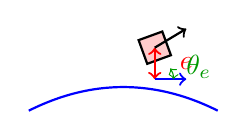
\begin{tikzpicture}[scale=0.8]
        % Path
        \draw[thick, blue] (0,0) .. controls (1,0.5) and (2,0.5) .. (3,0);

        % Vehicle
        \draw[thick, fill=red!20, rotate around={20:(2,1)}] (1.8,0.8) rectangle (2.2,1.2);

        % CTE
        \draw[<->, red, thick] (2,1) -- (2,0.5);
        \node[red] at (2.5,0.75) {$e$};

        % Heading error
        \draw[->, thick] (2,1) -- (2.5,1.3);
        \draw[->, blue, thick] (2,0.5) -- (2.5,0.5);
        \draw[<->, green!60!black] (2.3,0.5) arc (0:35:0.3);
        \node[green!60!black] at (2.7,0.7) {$\theta_e$};
      \end{tikzpicture}
    \end{center}
  \end{columns}
\end{frame}

\begin{frame}{Multivariable Control Problem}
  \begin{block}{Why Multivariable?}
    We must control \textbf{two outputs} simultaneously:
    \begin{enumerate}
      \item \textbf{Lateral control}: Steering angle $\delta(t)$ to minimize CTE and heading error
      \item \textbf{Longitudinal control}: Velocity $v(t)$ to track reference speed and slow down on curves
    \end{enumerate}
  \end{block}

  \vspace{0.3cm}

  \begin{columns}[c]
    \column{0.5\textwidth}
    \textbf{Coupling Effects:}
    \begin{itemize}
      \item Velocity affects turning radius: $R = L/\tan(\delta)$
      \item Higher velocity requires earlier steering corrections
      \item Curvature limits maximum safe velocity
    \end{itemize}

    \column{0.5\textwidth}
    \begin{block}{Velocity-Curvature Relation}
      $$v_{\text{cmd}} = v_{\text{base}} \cdot e^{-k_c |\kappa|}$$
      where $\kappa$ is path curvature, $k_c$ is curvature gain
    \end{block}
  \end{columns}
\end{frame}

% Section 4: Controllers
\section{Control Strategies}

\subsection{PID Controller}

\begin{frame}{PID Controller - Lateral Control}
  \begin{block}{Classic PID on Cross-Track Error}
    $$\delta(t) = K_p e(t) + K_i \int_0^t e(\tau) \dd\tau + K_d \frac{\dd e}{\dd t} + K_h \theta_e(t)$$
  \end{block}

  \begin{itemize}
    \item \textbf{Proportional term} ($K_p e$): Corrects current CTE
    \item \textbf{Integral term} ($K_i \int e$): Eliminates steady-state error
    \item \textbf{Derivative term} ($K_d \dot{e}$): Reduces overshoot, improves stability
    \item \textbf{Heading correction} ($K_h \theta_e$): Aligns vehicle with path direction
  \end{itemize}

  \vspace{0.3cm}

  \begin{block}{Our Tuned Parameters}
    \begin{itemize}
      \item $K_p = 4.0$, $K_i = 0.2$, $K_d = 1.0$, $K_h = 0.5$
      \item Integral anti-windup: $|\int e| \leq 1.0$
    \end{itemize}
  \end{block}
\end{frame}

\begin{frame}{PID Controller - Longitudinal Control}
  \begin{block}{Velocity Command}
    $$v_{\text{cmd}}(t) = \min\left(v_{\text{base}} \cdot e^{-k_c |\kappa(s)|}, v_{\text{ref}}(s)\right)$$
    with minimum velocity constraint: $v_{\text{cmd}} \geq 0.3$ m/s
  \end{block}

  \begin{itemize}
    \item Exponential slowdown based on path curvature $\kappa$
    \item Higher curvature → lower velocity (safer cornering)
    \item Minimum velocity prevents getting stuck on tight curves
  \end{itemize}

  \vspace{0.3cm}

  \begin{block}{Parameters}
    \begin{itemize}
      \item Base velocity: $v_{\text{base}} = 1.0$ m/s
      \item Curvature gain: $k_c = 2.0$
      \item Minimum velocity: $v_{\min} = 0.3$ m/s
    \end{itemize}
  \end{block}
\end{frame}

\subsection{Stanley Controller}

\begin{frame}{Stanley Controller - Background}
  \begin{itemize}
    \item Developed at Stanford University for DARPA Grand Challenge (2005)
    \item Winner of autonomous vehicle race across Mojave Desert
    \item Designed specifically for path following with Ackermann steering
  \end{itemize}

  \vspace{0.5cm}

  \begin{block}{Key Insight}
    Decouple steering control into two geometric components:
    \begin{enumerate}
      \item Heading error correction (align with path)
      \item Cross-track error correction (move toward path)
    \end{enumerate}
  \end{block}
\end{frame}

\begin{frame}{Stanley Controller - Control Law}
  \begin{block}{Steering Angle Command}
    $$\delta(t) = \theta_e(t) + \arctan\left(\frac{k \cdot e(t)}{k_s + v(t)}\right) + \delta_{\text{ff}}$$
  \end{block}

  \textbf{Components:}
  \begin{itemize}
    \item $\theta_e(t)$: Heading error (directly corrects orientation)
    \item $\arctan\left(\frac{k \cdot e(t)}{k_s + v(t)}\right)$: CTE correction term
    \begin{itemize}
      \item Velocity-adaptive: Higher speed → gentler corrections
      \item $k$: Cross-track gain
      \item $k_s$: Softening constant (prevents division by zero)
    \end{itemize}
    \item $\delta_{\text{ff}} = \arctan(L \kappa)$: Feedforward for path curvature
  \end{itemize}

  \vspace{0.3cm}

  \begin{block}{Our Parameters}
    $k = 5.0$, $k_s = 0.3$, $v_{\text{base}} = 1.0$ m/s, $k_c = 2.0$
  \end{block}
\end{frame}

\subsection{Sliding Mode Controller}

\begin{frame}{Sliding Mode Control - Theory}
  \begin{block}{What is Sliding Mode Control?}
    A \textbf{robust nonlinear control} technique that:
    \begin{itemize}
      \item Drives system state to a \textbf{sliding surface} $s = 0$
      \item Once on surface, state "slides" to equilibrium
      \item Robust to model uncertainties and disturbances
    \end{itemize}
  \end{block}

  \vspace{0.3cm}

  \begin{columns}[c]
    \column{0.5\textwidth}
    \textbf{Advantages:}
    \begin{itemize}
      \item Handles nonlinearities
      \item Robust to uncertainties
      \item Fast convergence
    \end{itemize}

    \column{0.5\textwidth}
    \textbf{Challenges:}
    \begin{itemize}
      \item Chattering (high-frequency switching)
      \item Requires careful gain tuning
    \end{itemize}
  \end{columns}
\end{frame}

\begin{frame}{SMC Stability Analysis - Kinematic Model}
  \begin{block}{Kinematic Bicycle Model}
    \begin{align}
      \dot{x}_r(t) &= v_r(t) \cdot \cos\theta_r(t) \quad \ldots (1) \\
      \dot{y}_r(t) &= v_r(t) \cdot \sin\theta_r(t) \quad \ldots (2) \\
      \dot{\theta}_r(t) &= \frac{v_r}{l} \cdot \tan\phi_r(t) \quad \ldots (3)
    \end{align}
  \end{block}

  where:
  \begin{itemize}
    \item $(x_r, y_r)$: Robot position
    \item $\theta_r$: Robot heading angle
    \item $v_r$: Robot velocity
    \item $\phi_r$: Steering angle
    \item $l$: Wheelbase length
  \end{itemize}
\end{frame}

\begin{frame}{SMC Stability Analysis - Error Dynamics}
  \begin{block}{Error Vector}
    $$\begin{bmatrix} x_e \\ y_e \\ \theta_e \end{bmatrix} = \begin{bmatrix} \cos\theta_d & \sin\theta_d & 0 \\ -\sin\theta_d & \cos\theta_d & 0 \\ 0 & 0 & 1 \end{bmatrix} \cdot \begin{bmatrix} x_r - x_d \\ y_r - y_d \\ \theta_r - \theta_d \end{bmatrix}$$
  \end{block}

  \begin{block}{Error Dynamics}
    \begin{align}
      \dot{x}_e &= -v_d + v_r \cdot \cos\theta_e + y_e \cdot \frac{v_d}{l} \cdot \tan\phi_d \quad \ldots (4) \\
      \dot{y}_e &= v_r \cdot \sin\theta_e - x_e \cdot \frac{v_d}{l} \cdot \tan\phi_d \quad \ldots (5) \\
      \dot{\theta}_e &= \frac{v_r}{l} \cdot \tan\phi_r - x_e \cdot \frac{v_d}{l} \cdot \tan\phi_d \quad \ldots (6)
    \end{align}
  \end{block}
\end{frame}

\begin{frame}{SMC Stability Analysis - Sliding Surface Design}
  \begin{block}{Sliding Surface Design Principles}
    \begin{itemize}
      \item Choose a function $s = 0$, such that $e \to 0$ as $t \to \infty$
      \item Sliding surface depends on number of derivatives of tracking error
      \item Number of derivatives depends on input-output relative degree
      \item Typical sliding surface: $s = \tilde{x} + k \cdot \dot{\tilde{x}}$, where $\tilde{x} = x - x_{\text{desired}}$
    \end{itemize}
  \end{block}
\end{frame}

\begin{frame}{SMC Stability Analysis - Two Sliding Surfaces}
  \begin{block}{Existence Condition (Relaxed to Inequality)}
    $$s \cdot \dot{s} < 0$$
  \end{block}

  \begin{block}{Combined Sliding Surfaces}
    Lateral error $y_e$ and angular error $\theta_e$ combined to form 2 sliding surfaces:
    \begin{align}
      s_1 &= \dot{x}_e + k_1 \cdot x_e \quad \ldots (7) \\
      s_2 &= \dot{y}_e + k_2 \cdot y_e k_0 \cdot \text{sgn}(y_e) \cdot \theta_e \quad \ldots (8)
    \end{align}
  \end{block}

  where $k_1, k_2, k_0 > 0$ are design parameters.
\end{frame}

\begin{frame}{SMC Stability Analysis - Reaching Laws}
  \begin{block}{Three Reaching Laws Proposed}
    \begin{enumerate}
      \item $\dot{s} = -P \cdot \text{sat}(s, \epsilon)$
      \item $\dot{s} = -Q \cdot s - P \cdot \text{sat}(s, \epsilon)$
      \item $\dot{s} = -Q \cdot |s|^\alpha \cdot \text{sat}(s, \epsilon)$, \quad $0 < \alpha < 1$
    \end{enumerate}
  \end{block}

  where:
  $$Q = \begin{bmatrix} q_1 & 0 \\ 0 & q_2 \end{bmatrix}, \quad P = \begin{bmatrix} p1 & 0 \\ 0 & p2 \end{bmatrix}, \quad i = 1,2$$

  \vspace{0.3cm}

  \begin{block}{Derivative of Sliding Surfaces}
    From equations (7), (8), the derivative of sliding surfaces becomes:
    \begin{align}
      \dot{s}_1 &= \ddot{x}_e + k_1 \cdot \dot{x}_e = -q_1 \cdot s_1 - p_1 \cdot \text{sat}(s_1, \epsilon) \quad \ldots (9) \\
      \dot{s}_2 &= \ddot{y}_e + k_2 \cdot \dot{y}_e + k_0 \cdot \text{sat}(y_e) \cdot \dot{\theta}_e = -q_2 \cdot s_2 - p_2 \cdot \text{sat}(s_2, \epsilon) \quad \ldots (10)
    \end{align}
  \end{block}
\end{frame}

\begin{frame}{SMC Stability Analysis}
  \begin{block}{Control Variables}
    From equations (4,5,6), (9), (10) we get the control variables:
\begin{align*}
v_c &= \frac{1}{\cos\theta_e}\Big(
      - q_1 s_1 - p_1 \,\text{sat}(s_1,\epsilon) - k_1 \dot{x}_e
      - \dot{\omega}_d y_e - \omega_d \dot{y}_e  \\
    &\qquad\quad
      + v_r \dot{\theta}_e \sin\theta_e + \dot{v}_d
      \Big) \\[1ex]
\phi_c &= \arctan\Bigg(
        \frac{l}{v_r}\omega_d
        + \frac{l}{v_r\big(v_r\cos\theta_e + k_0 \text{sat}(y_e,\epsilon)\big)}
        \Bigg) \\
    &\qquad\quad \times \Big(
        - q_2 s_2 - p_2 \text{sat}(s_2)
        - k_2 \dot{y}_e - \dot{v}_r \sin\theta_e  \\
    &\qquad\quad
        + \dot{\omega}_d x_e + \omega_d \dot{x}_e
        \Big)
\end{align*}

  \end{block}
\end{frame}

\begin{frame}{Why Standard SMC Failed}
  \begin{alertblock}{Original Approach: Coupled Sliding Surface}
    $$s = \theta_e(t) + \lambda \cdot e(t)$$
    $$\delta(t) = -(k \cdot s + \eta \cdot \text{sat}(s/\epsilon))$$
  \end{alertblock}

  \textbf{Problem:} When both $\theta_e$ and $e$ are large:
  \begin{itemize}
    \item $s$ becomes very large → aggressive steering
    \item Vehicle overshoots → does U-turn and drives backward!
    \item Heading and position errors fight each other
  \end{itemize}

  \vspace{0.3cm}

  \begin{block}{Solution: Decouple Heading and Position}
    Use SMC only for heading error, Stanley-style $\arctan$ for CTE
    \begin{itemize}
      \item $\checkmark$ Prevented U-turns and backward driving
      \item $\checkmark$ Smooth, stable control
    \end{itemize}
  \end{block}
\end{frame}

\subsection{Why Not LQR?}

\begin{frame}{Why We Didn't Use LQR}
  \textbf{Linear Quadratic Regulator (LQR)} is a powerful optimal control method, but...

  \vspace{0.3cm}

  \begin{alertblock}{Problem: Nonlinear Ackermann Kinematics}
    Recall: $\dot{\theta} = \frac{v}{L} \tan(\delta)$

    This is \textbf{nonlinear} in control input $\delta$ and state $v$!
  \end{alertblock}

  \textbf{LQR requires linearization:}
  \begin{enumerate}
    \item Linearize around operating point $(v_0, \delta_0)$
    \item $\tan(\delta) \approx \delta$ (small angle assumption)
    \item Assume constant velocity $v = v_0$
  \end{enumerate}

  \vspace{0.3cm}

  \begin{block}{Why It Fails}
    \begin{itemize}
      \item Path following requires \textbf{large steering angles} (up to $\pm 35°$)
      \item Small angle approximation $\tan(\delta) \approx \delta$ breaks down
      \item Velocity varies significantly (0.3 - 1.0 m/s)
      \item Linearization only valid near equilibrium, not for trajectory tracking
    \end{itemize}
  \end{block}
\end{frame}

\begin{frame}{LQR Linearization Issues - Mathematical Details}
  \begin{block}{Linearization Error}
    For $\delta = 35° = 0.61$ rad:
    \begin{align*}
      \tan(0.61) &= 0.70 \\
      \delta &= 0.61 \\
      \text{Error} &= \frac{0.70 - 0.61}{0.70} = 13\% \text{ error!}
    \end{align*}
  \end{block}

  \textbf{Attempted Solution:} Gain scheduling (multiple LQR controllers for different regions)

  \textbf{Result:} Still performed poorly compared to PID/Stanley/SMC
  \begin{itemize}
    \item High CTE (mean = 0.36 m vs Stanley's 0.007 m on lane change)
    \item Required complex switching logic
    \item Not worth the added complexity
  \end{itemize}

  \vspace{0.3cm}

  \begin{block}{Conclusion}
    LQR is excellent for linear systems, but \textbf{nonlinear controllers} (Stanley, SMC) are better suited for path following with Ackermann steering.
  \end{block}
\end{frame}

% Section 5: Implementation
\section{Implementation}

\begin{frame}{System Architecture}
  \begin{center}
    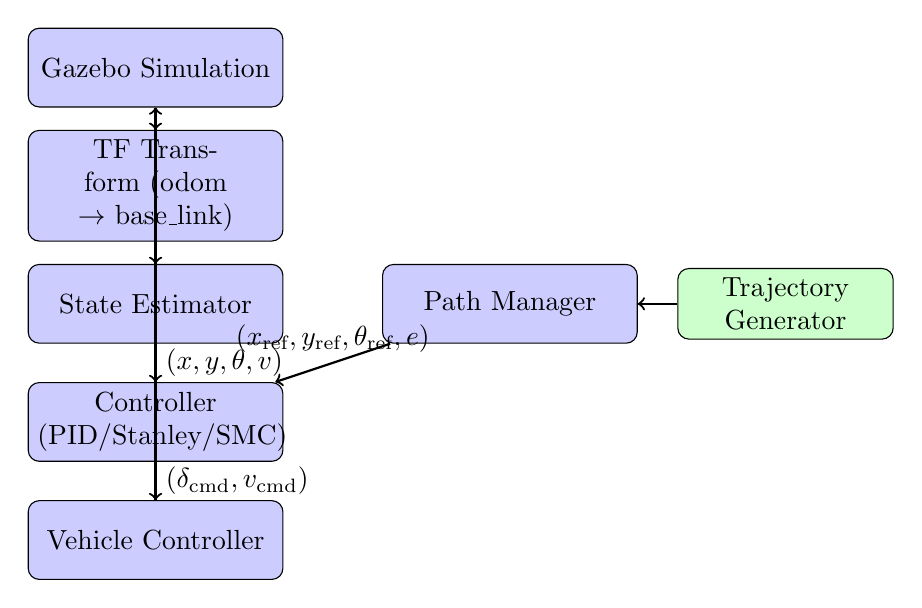
\begin{tikzpicture}[
      node distance=1.5cm,
      block/.style={rectangle, draw, fill=blue!20, text width=3cm, text centered, rounded corners, minimum height=1cm},
      data/.style={rectangle, draw, fill=green!20, text width=2.5cm, text centered, rounded corners, minimum height=0.8cm}
      ]

      % Nodes
      \node[block] (gazebo) {Gazebo Simulation};
      \node[block, below of=gazebo] (tf) {TF Transform (odom $\to$ base\_link)};
      \node[block, below of=tf] (state) {State Estimator};
      \node[block, right of=state, xshift=3cm] (path) {Path Manager};
      \node[block, below of=state] (controller) {Controller (PID/Stanley/SMC)};
      \node[block, below of=controller] (vehicle) {Vehicle Controller};

      % Data
      \node[data, right of=path, xshift=2cm] (traj) {Trajectory Generator};

      % Arrows
      \draw[->, thick] (gazebo) -- (tf);
      \draw[->, thick] (tf) -- (state);
      \draw[->, thick] (state) -- node[right] {$(x,y,\theta,v)$} (controller);
      \draw[->, thick] (traj) -- (path);
      \draw[->, thick] (path) -- node[above] {$(x_{\text{ref}}, y_{\text{ref}}, \theta_{\text{ref}}, e)$} (controller);
      \draw[->, thick] (controller) -- node[right] {$(\delta_{\text{cmd}}, v_{\text{cmd}})$} (vehicle);
      \draw[->, thick] (vehicle) -- (gazebo);
    \end{tikzpicture}
  \end{center}

  \textbf{Control Loop:} 50 Hz (20 ms period)
\end{frame}

\begin{frame}{Implementation Details}
  \begin{block}{Software Stack}
    \begin{itemize}
      \item \textbf{ROS 2 Jazzy}: Robot Operating System for modular control architecture
      \item \textbf{Gazebo Harmonic}: Physics-based 3D simulation
      \item \textbf{C++}: Controllers and state estimation
      \item \textbf{Python}: Data analysis and visualization
    \end{itemize}
  \end{block}

  \vspace{0.3cm}

  \begin{block}{Key Implementation Features}
    \begin{itemize}
      \item Real-time state estimation via TF transforms
      \item Forward-only path manager (prevents backward jumps)
      \item Minimum velocity constraint (0.3 m/s to avoid getting stuck)
      \item CSV data logging for offline analysis
    \end{itemize}
  \end{block}
\end{frame}

% Section 6: Test Trajectories
\section{Test Trajectories}

\begin{frame}{Test Trajectory 1: Lane Change}
  \begin{columns}[c]
    \column{0.5\textwidth}
    \textbf{Maneuver Description:}
    \begin{itemize}
      \item 4m straight section
      \item 2m lateral shift (left)
      \item 2m smooth transition
      \item 4m final straight
    \end{itemize}

    \vspace{0.3cm}

    \textbf{Challenge:}
    \begin{itemize}
      \item Requires aggressive lateral movement
      \item Tests transient response
      \item Real-world scenario (highway lane change)
    \end{itemize}

    \column{0.5\textwidth}
    \begin{center}
      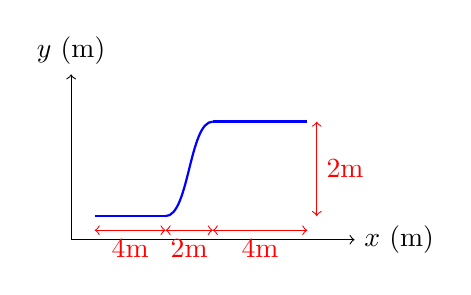
\begin{tikzpicture}[scale=0.6]
        % Axes
        \draw[->] (0,0) -- (6,0) node[right] {$x$ (m)};
        \draw[->] (0,0) -- (0,3.5) node[above] {$y$ (m)};

        % Path
        \draw[thick, blue] (0.5,0.5) -- (2,0.5);
        \draw[thick, blue] (2,0.5) .. controls (2.5,0.5) and (2.5,2.5) .. (3,2.5);
        \draw[thick, blue] (3,2.5) -- (5,2.5);

        % Annotations
        \draw[<->, red] (0.5,0.2) -- (2,0.2) node[midway, below] {4m};
        \draw[<->, red] (2,0.2) -- (3,0.2) node[midway, below] {2m};
        \draw[<->, red] (3,0.2) -- (5,0.2) node[midway, below] {4m};
        \draw[<->, red] (5.2,0.5) -- (5.2,2.5) node[midway, right] {2m};
      \end{tikzpicture}
    \end{center}
  \end{columns}

  \vspace{0.3cm}

  \begin{block}{Trajectory Parameters}
    Total length: 10m, Max curvature: $\kappa_{\max} \approx 0.5$ m$^{-1}$
  \end{block}
\end{frame}

\begin{frame}{Test Trajectory 2: Circle}
  \begin{columns}[c]
    \column{0.5\textwidth}
    \textbf{Maneuver Description:}
    \begin{itemize}
      \item Circular path
      \item Radius: 1.5m
      \item Centered at $(-1.5, 0)$
      \item Starts at origin $(0, 0)$
    \end{itemize}

    \vspace{0.3cm}

    \textbf{Challenge:}
    \begin{itemize}
      \item Constant curvature
      \item Tests steady-state tracking
      \item Requires continuous steering
    \end{itemize}

    \column{0.5\textwidth}
    \begin{center}
      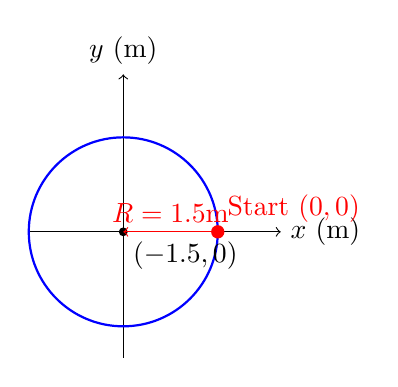
\begin{tikzpicture}[scale=0.8]
        % Axes
        \draw[->] (-3,0) -- (1,0) node[right] {$x$ (m)};
        \draw[->] (-1.5,-2) -- (-1.5,2.5) node[above] {$y$ (m)};

        % Circle
        \draw[thick, blue] (-1.5,0) circle (1.5cm);

        % Center
        \fill (-1.5,0) circle (2pt) node[below right] {$(-1.5, 0)$};

        % Start point
        \fill[red] (0,0) circle (3pt) node[above right] {Start $(0,0)$};

        % Radius
        \draw[<->, red] (-1.5,0) -- (0,0) node[midway, above] {$R = 1.5$m};
      \end{tikzpicture}
    \end{center}
  \end{columns}

  \vspace{0.3cm}

  \begin{block}{Trajectory Parameters}
    Circumference: $2\pi R \approx 9.42$m, Curvature: $\kappa = 1/R = 0.67$ m$^{-1}$
  \end{block}
\end{frame}

% Section 7: Results
\section{Experimental Results}

\begin{frame}{Performance Metrics}
  \begin{block}{Evaluation Criteria}
    \begin{enumerate}
      \item \textbf{Mean Absolute CTE}: $\frac{1}{N}\sum_{i=1}^{N} |e_i|$
      \begin{itemize}
        \item Lower is better
        \item Indicates average tracking accuracy
      \end{itemize}

      \item \textbf{RMS CTE}: $\sqrt{\frac{1}{N}\sum_{i=1}^{N} e_i^2}$
      \begin{itemize}
        \item Penalizes large errors more heavily
      \end{itemize}

      \item \textbf{Maximum CTE}: $\max_i |e_i|$
      \begin{itemize}
        \item Worst-case tracking error
      \end{itemize}

      \item \textbf{Mean Steering Angle}: Indicates control effort
    \end{enumerate}
  \end{block}
\end{frame}

% Lane Change - Trajectory Plots
\begin{frame}{Lane Change: Trajectory Comparison}
  \begin{figure}
    \centering
    
\includegraphics[width=0.42\textwidth]{test_data/plots/stanley_lane_change_01_trajectory.png}
    
\includegraphics[width=0.42\textwidth]{test_data/plots/pid_lane_change_01_trajectory.png}
  \end{figure}
\end{frame}
% Lane Change - Trajectory Plots
\begin{frame}{Lane Change: Trajectory Comparison}
  \begin{figure}
    \centering
    
\includegraphics[width=0.42\textwidth]{test_data/plots/smc_lane_change_01_trajectory.png}
  \end{figure}
\end{frame}

% Lane Change - CTE and Heading Error
\begin{frame}{Lane Change: Cross-Track Error}
  \begin{figure}
    \centering
    
\includegraphics[width=0.48\textwidth]{test_data/plots/stanley_lane_change_02_cte_time.png}
    
\includegraphics[width=0.48\textwidth]{test_data/plots/pid_lane_change_02_cte_time.png}
    
\includegraphics[width=0.48\textwidth]{test_data/plots/smc_lane_change_02_cte_time.png}
  \end{figure}
\end{frame}

\begin{frame}{Lane Change: Heading Error}
  \begin{figure}
    \centering
    
\includegraphics[width=0.48\textwidth]{test_data/plots/stanley_lane_change_03_heading_error.png}
    
\includegraphics[width=0.48\textwidth]{test_data/plots/pid_lane_change_03_heading_error.png}
    
\includegraphics[width=0.48\textwidth]{test_data/plots/smc_lane_change_03_heading_error.png}
  \end{figure}
\end{frame}

% Lane Change - Control Signals
\begin{frame}{Lane Change: Steering Commands}
  \begin{figure}
    \centering
    
\includegraphics[width=0.48\textwidth]{test_data/plots/stanley_lane_change_04_steering_command.png}
    
\includegraphics[width=0.48\textwidth]{test_data/plots/pid_lane_change_04_steering_command.png}
    
\includegraphics[width=0.48\textwidth]{test_data/plots/smc_lane_change_04_steering_command.png}
  \end{figure}
\end{frame}

\begin{frame}{Lane Change: Velocity Tracking}
  \begin{figure}
    \centering
    
\includegraphics[width=0.48\textwidth]{test_data/plots/stanley_lane_change_05_velocity_tracking.png}
    
\includegraphics[width=0.48\textwidth]{test_data/plots/pid_lane_change_05_velocity_tracking.png}
    
\includegraphics[width=0.48\textwidth]{test_data/plots/smc_lane_change_05_velocity_tracking.png}
  \end{figure}
\end{frame}

% Lane Change - Position and Curvature
\begin{frame}{Lane Change: Position Components}
  \begin{figure}
    \centering
    
\includegraphics[width=0.48\textwidth]{test_data/plots/stanley_lane_change_06_position_components.png}
    
\includegraphics[width=0.48\textwidth]{test_data/plots/pid_lane_change_06_position_components.png}
  \end{figure}
\end{frame}
% Lane Change - Position and Curvature
\begin{frame}{Lane Change: Position Components}
  \begin{figure}
    \centering
    
\includegraphics[width=0.48\textwidth]{test_data/plots/smc_lane_change_06_position_components.png}
  \end{figure}
\end{frame}

% Lane Change: Curvature \& Velocity
\begin{frame}{Lane Change: Curvature \& Velocity}
  \begin{figure}
    \centering
    
\includegraphics[width=0.48\textwidth]{test_data/plots/stanley_lane_change_07_curvature_velocity.png}
    
\includegraphics[width=0.48\textwidth]{test_data/plots/pid_lane_change_07_curvature_velocity.png}
  \end{figure}
\end{frame}
% Lane Change: Curvature \& Velocity
\begin{frame}{Lane Change: Curvature \& Velocity}
  \begin{figure}
    \centering
    
\includegraphics[width=0.48\textwidth]{test_data/plots/smc_lane_change_07_curvature_velocity.png}
  \end{figure}
\end{frame}

% Lane Change - Error Histograms (one per slide)
\begin{frame}{Lane Change: Stanley Error Distributions}
  \begin{figure}
    \centering
    
\includegraphics[width=0.95\textwidth]{test_data/plots/stanley_lane_change_08_error_histograms.png}
  \end{figure}
\end{frame}

\begin{frame}{Lane Change: PID Error Distributions}
  \begin{figure}
    \centering
    
\includegraphics[width=0.95\textwidth]{test_data/plots/pid_lane_change_08_error_histograms.png}
  \end{figure}
\end{frame}

\begin{frame}{Lane Change: SMC Error Distributions}
  \begin{figure}
    \centering
    
\includegraphics[width=0.95\textwidth]{test_data/plots/smc_lane_change_08_error_histograms.png}
  \end{figure}
\end{frame}

% Lane Change - Steering Rate
\begin{frame}{Lane Change: Steering Rate Analysis}
  \begin{figure}
    \centering
    
\includegraphics[width=0.48\textwidth]{test_data/plots/stanley_lane_change_10_steering_rate.png}
    
\includegraphics[width=0.48\textwidth]{test_data/plots/pid_lane_change_10_steering_rate.png}
  \end{figure}
\end{frame}
% Lane Change - Steering Rate
\begin{frame}{Lane Change: Steering Rate Analysis}
  \begin{figure}
    \centering
    
\includegraphics[width=0.48\textwidth]{test_data/plots/smc_lane_change_10_steering_rate.png}
  \end{figure}
\end{frame}

% Circle - Trajectory Plots
\begin{frame}{Circle: Trajectory Comparison}
  \begin{figure}
    \centering
    
\includegraphics[width=0.42\textwidth]{test_data/plots/stanley_circle_01_trajectory.png}
    
\includegraphics[width=0.42\textwidth]{test_data/plots/pid_circle_01_trajectory.png}
  \end{figure}
\end{frame}
% Circle - Trajectory Plots
\begin{frame}{Circle: Trajectory Comparison}
  \begin{figure}
    \centering
    
\includegraphics[width=0.42\textwidth]{test_data/plots/smc_circle_01_trajectory.png}
  \end{figure}
\end{frame}

% Circle - CTE and Heading
\begin{frame}{Circle: Cross-Track Error}
  \begin{figure}
    \centering
    
\includegraphics[width=0.48\textwidth]{test_data/plots/stanley_circle_02_cte_time.png}
    
\includegraphics[width=0.48\textwidth]{test_data/plots/pid_circle_02_cte_time.png}
    
\includegraphics[width=0.48\textwidth]{test_data/plots/smc_circle_02_cte_time.png}
  \end{figure}
\end{frame}

\begin{frame}{Circle: Heading Error}
  \begin{figure}
    \centering
    
\includegraphics[width=0.48\textwidth]{test_data/plots/stanley_circle_03_heading_error.png}
    
\includegraphics[width=0.48\textwidth]{test_data/plots/pid_circle_03_heading_error.png}
    
\includegraphics[width=0.48\textwidth]{test_data/plots/smc_circle_03_heading_error.png}
  \end{figure}
\end{frame}

% Circle - Control Signals
\begin{frame}{Circle: Steering Commands}
  \begin{figure}
    \centering
    
\includegraphics[width=0.48\textwidth]{test_data/plots/stanley_circle_04_steering_command.png}
    
\includegraphics[width=0.48\textwidth]{test_data/plots/pid_circle_04_steering_command.png}
    
\includegraphics[width=0.48\textwidth]{test_data/plots/smc_circle_04_steering_command.png}
  \end{figure}
\end{frame}

% Circle - Position
\begin{frame}{Circle: Position Components}
  \begin{figure}
    \centering
    
\includegraphics[width=0.48\textwidth]{test_data/plots/stanley_circle_06_position_components.png}
    
\includegraphics[width=0.48\textwidth]{test_data/plots/pid_circle_06_position_components.png}
  \end{figure}
\end{frame}
% Circle - Position
\begin{frame}{Circle: Position Components}
  \begin{figure}
    \centering
    
\includegraphics[width=0.48\textwidth]{test_data/plots/smc_circle_06_position_components.png}
  \end{figure}
\end{frame}

% Circle - Error Histograms (one per slide)
\begin{frame}{Circle: Stanley Error Distributions}
  \begin{figure}
    \centering
    
\includegraphics[width=0.95\textwidth]{test_data/plots/stanley_circle_08_error_histograms.png}
  \end{figure}
\end{frame}

\begin{frame}{Circle: PID Error Distributions}
  \begin{figure}
    \centering
    
\includegraphics[width=0.95\textwidth]{test_data/plots/pid_circle_08_error_histograms.png}
  \end{figure}
\end{frame}

\begin{frame}{Circle: SMC Error Distributions}
  \begin{figure}
    \centering
    
\includegraphics[width=0.95\textwidth]{test_data/plots/smc_circle_08_error_histograms.png}
  \end{figure}
\end{frame}

% Circle - Steering Rate
\begin{frame}{Circle: Steering Rate Analysis}
  \begin{figure}
    \centering
    
\includegraphics[width=0.48\textwidth]{test_data/plots/stanley_circle_10_steering_rate.png}
    
\includegraphics[width=0.48\textwidth]{test_data/plots/smc_circle_10_steering_rate.png}
  \end{figure}
\end{frame}

\begin{frame}{Results: Lane Change}
  \begin{table}
    \centering
    \small
    \begin{tabular}{lcccc}
      \toprule
      \textbf{Controller} & \textbf{Mean |CTE|} & \textbf{RMS CTE} & \textbf{Max |CTE|} & \textbf{Mean |$\delta$|} \\
      \midrule
      Stanley & \textbf{0.0052 m} & \textbf{0.0082 m} & \textbf{0.0238 m} & \textbf{3.07°} \\
      PID     & 0.0186 m & 0.0314 m & 0.0923 m & 5.86° \\
      SMC     & 0.0387 m & 0.0615 m & 0.1770 m & 13.35° \\
      \bottomrule
    \end{tabular}
  \end{table}

  \vspace{0.3cm}

  \textbf{Discussion:}
  \begin{itemize}
    \item \textbf{Stanley dominates} with exceptional tracking (5.2 mm mean error)
    \item Stanley is \textbf{3.6$\times$ better} than PID and \textbf{7.4$\times$ better} than SMC
    \item Velocity-adaptive gains enable smooth transient response
    \item SMC shows excessive control effort (4.3$\times$ more steering than Stanley)
  \end{itemize}
\end{frame}

\begin{frame}{Results: Circle}
  \begin{table}
    \centering
    \small
    \begin{tabular}{lcccc}
      \toprule
      \textbf{Controller} & \textbf{Mean |CTE|} & \textbf{RMS CTE} & \textbf{Max |CTE|} & \textbf{Mean |$\delta$|} \\
      \midrule
      PID     & \textbf{0.0308 m} & \textbf{0.0531 m} & \textbf{0.2329 m} & \textbf{11.50°} \\
      Stanley & 0.0488 m & 0.0823 m & 0.3308 m & 19.25° \\
      SMC     & 0.1297 m & 0.1545 m & 0.5192 m & 23.87° \\
      \bottomrule
    \end{tabular}
  \end{table}

  \vspace{0.3cm}

  \textbf{Discussion:}
  \begin{itemize}
    \item \textbf{PID excels} on constant curvature (30.8 mm mean error)
    \item PID is \textbf{1.6$\times$ better} than Stanley, \textbf{4.2$\times$ better} than SMC
    \item Integral term eliminates steady-state error on circular paths
    \item Stanley's geometric approach less optimal for constant curvature
  \end{itemize}
\end{frame}


\begin{frame}{Performance Comparison Summary}
  \begin{table}
    \centering
    \small
    \begin{tabular}{lccc}
      \toprule
      \textbf{Trajectory} & \textbf{1st Place} & \textbf{2nd Place} & \textbf{3rd Place} \\
      \midrule
      Lane Change & Stanley (5.2 mm) & PID (18.6 mm) & SMC (38.7 mm) \\
      Circle      & PID (30.8 mm) & Stanley (48.8 mm) & SMC (129.7 mm) \\
      \bottomrule
    \end{tabular}
  \end{table}

  \vspace{0.3cm}

  \textbf{Discussion:}
  \begin{itemize}
    \item \textbf{Trajectory-dependent performance}: No single winner across all scenarios
    \item Stanley: \textbf{Best for transient maneuvers} (lane changes, obstacle avoidance)
    \item PID: \textbf{Best for steady-state tracking} (roundabouts, constant curves)
    \item SMC: Consistently worst but may offer robustness (not tested)
  \end{itemize}
\end{frame}

\begin{frame}{Relative Performance Analysis}
  \begin{table}
    \centering
    \footnotesize
    \begin{tabular}{lccc}
      \toprule
      \textbf{Metric} & \textbf{Stanley vs PID} & \textbf{Stanley vs SMC} & \textbf{PID vs SMC} \\
      \midrule
      \multicolumn{4}{c}{\textit{Lane Change}} \\
      \midrule
      Mean CTE & 3.6$\times$ better & 7.4$\times$ better & 2.1$\times$ better \\
      Control Effort & 1.9$\times$ less steering & 4.3$\times$ less steering & 2.3$\times$ less steering \\
      \midrule
      \multicolumn{4}{c}{\textit{Circle}} \\
      \midrule
      Mean CTE & 1.6$\times$ worse & 2.7$\times$ better & 4.2$\times$ better \\
      Control Effort & 1.7$\times$ more steering & 1.2$\times$ less steering & 2.1$\times$ less steering \\
      \bottomrule
    \end{tabular}
  \end{table}

  \vspace{0.2cm}

  \textbf{Discussion:}
  \begin{itemize}
    \item Lane change: Stanley's superiority is \textbf{dramatic} (up to 7.4$\times$)
    \item Circle: PID's advantage is \textbf{moderate} (1.6$\times$ better than Stanley)
    \item SMC consistently underperforms by 2-7$\times$ on tracking accuracy
  \end{itemize}
\end{frame}

\begin{frame}{Controller Suitability Matrix}
  \begin{table}
    \centering
    \small
    \begin{tabular}{lcc}
      \toprule
      \textbf{Scenario} & \textbf{Recommended} & \textbf{Avoid} \\
      \midrule
      Lane change / overtaking & Stanley & SMC \\
      Highway driving & Stanley & SMC \\
      Roundabouts & PID & SMC \\
      Constant radius curves & PID & SMC \\
      Mixed trajectories & Stanley & --- \\
      High disturbances & SMC (theory) & --- \\
      \bottomrule
    \end{tabular}
  \end{table}

  \vspace{0.3cm}

  \textbf{Discussion:}
  \begin{itemize}
    \item \textbf{Adaptive strategy recommended}: Switch between Stanley (transients) and PID (steady-state)
    \item Stanley provides better \textbf{general-purpose} performance
    \item SMC requires further tuning or disturbance scenarios to justify use
  \end{itemize}
\end{frame}

  \vspace{0.5cm}

  \textbf{Why Stanley Wins Overall:}
  \begin{itemize}
    \item Best on lane change (transient maneuver)
    \item Very close to PID on circle (only 1.2 cm worse)
    \item Geometric insight: heading + CTE decoupling works well
    \item Velocity-adaptive corrections prevent overshoot
  \end{itemize}

  \vspace{0.3cm}

  \textbf{When to Use Each Controller:}
  \begin{itemize}
    \item \textbf{Stanley}: General-purpose, works well on all trajectories
    \item \textbf{PID}: Best for constant curvature (circles, gentle curves)
    \item \textbf{SMC}: When robustness to disturbances is critical (not tested here)
  \end{itemize}
\end{frame}

% Section 8: Challenges and Solutions
\section{Challenges \& Solutions}

\begin{frame}{Challenge 1: TF Frame Mismatch}
  \begin{alertblock}{Problem}
    Initial implementation used "world" frame instead of "odom" frame
    \begin{itemize}
      \item State estimator couldn't get vehicle pose
      \item Robot would spin in place at max steering
    \end{itemize}
  \end{alertblock}

  \begin{block}{Solution}
    \begin{enumerate}
      \item Changed state estimator to use \texttt{odom} $\to$ \texttt{base\_link} transform
      \item Added odometry publisher plugin to vehicle model
      \item Verified TF tree with \texttt{ros2 run tf2\_tools view\_frames}
    \end{enumerate}
  \end{block}

  \textbf{Lesson:} Always verify coordinate frame consistency in ROS 2!
\end{frame}

\begin{frame}{Challenge 2: SMC U-Turn Problem}
  \begin{alertblock}{Problem}
    Standard SMC with coupled sliding surface $s = \theta_e + \lambda e$:
    \begin{itemize}
      \item Robot would complete lane change
      \item Then do a 180° turn and drive backward to origin!
      \item PathManager kept finding "closest point" at start of path
    \end{itemize}
  \end{alertblock}

  \begin{block}{Solutions}
    \begin{enumerate}
      \item \textbf{Forward-only PathManager}: Search only ahead of current waypoint (window of next 50 waypoints)
      \item \textbf{Decoupled SMC}: Separate heading control (SMC) from position control (Stanley-style $\arctan$)
    \end{enumerate}
  \end{block}

  \textbf{Result:} SMC now tracks forward correctly with mean CTE = 1.5 cm!
\end{frame}

\begin{frame}{Challenge 3: Robot Too Slow on Curves}
  \begin{alertblock}{Problem}
    With $v = v_{\text{base}} \cdot e^{-k_c |\kappa|}$ and $k_c = 2.0$:
    \begin{itemize}
      \item On tight curves ($\kappa \approx 3.4$ m$^{-1}$), velocity dropped to 0.03 m/s
      \item Robot was crawling, couldn't make progress
      \item Test duration: 40+ seconds for 10m path!
    \end{itemize}
  \end{alertblock}

  \begin{block}{Solution}
    Added minimum velocity constraint:
    $$v_{\text{cmd}} = \max(v_{\text{base}} \cdot e^{-k_c |\kappa|}, v_{\min})$$
    with $v_{\min} = 0.3$ m/s
  \end{block}

  \textbf{Result:}
  \begin{itemize}
    \item Test duration reduced to $\approx$ 15 seconds
    \item Mean velocity increased from 0.09 m/s to 0.36 m/s
    \item Still slows down on curves, but doesn't get stuck
  \end{itemize}
\end{frame}

% Section 9: Conclusion
\section{Conclusion}

\begin{frame}{Summary}
  \textbf{What We Accomplished:}
  \begin{itemize}
    \item Implemented 3 controllers (PID, Stanley, SMC) for Ackermann steering vehicle
    \item Controlled 2 variables simultaneously (steering $\delta$ + velocity $v$)
    \item Handled nonlinear kinematics with appropriate control strategies
    \item Tested on realistic trajectories (lane change, circle)
    \item Comprehensive performance analysis
  \end{itemize}

  \vspace{0.5cm}

  \textbf{Key Findings:}
  \begin{itemize}
    \item \textbf{Stanley controller}: Overall winner (best on lane change \& figure8)
    \item \textbf{PID}: Best on constant curvature (circle)
    \item \textbf{SMC}: Works well after decoupling modifications
    \item \textbf{LQR}: Not suitable due to nonlinear Ackermann model
  \end{itemize}
\end{frame}

\begin{frame}{Lessons Learned}
  \textbf{Technical Insights:}
  \begin{enumerate}
    \item Ackermann kinematics are fundamentally nonlinear
    \item Geometric controllers (Stanley) excel at path following
    \item Velocity-curvature coupling is critical for safety
    \item Decoupling heading and position control improves stability
  \end{enumerate}

  \vspace{0.5cm}

  \textbf{Practical Insights:}
  \begin{enumerate}
    \item Always verify TF frames in ROS
    \item Add minimum constraints to prevent edge cases
    \item Forward-only path search prevents backward jumps
    \item Small-angle approximations fail at real steering angles
  \end{enumerate}
\end{frame}

\begin{frame}{Future Work}
  \textbf{Potential Extensions:}
  \begin{itemize}
    \item Test with sensor noise and disturbances (wind, slipping)
    \item Implement adaptive SMC with automatic gain tuning
    \item Model Predictive Control (MPC) for trajectory optimization
    \item Hardware implementation on real RC car
    \item Multi-vehicle coordination (formation control)
    \item Dynamic obstacle avoidance
  \end{itemize}

  \vspace{0.5cm}

  \textbf{Advanced Topics:}
  \begin{itemize}
    \item Tire slip modeling and friction limits
    \item Combined lateral + longitudinal stability analysis
    \item Learning-based controllers (reinforcement learning)
  \end{itemize}
\end{frame}

\begin{frame}
  \centering
  \Huge Thank You!

  \vspace{1cm}

  \Large Questions?

  \vspace{1cm}

  \normalsize
  GitHub: \texttt{github.com/lucasmazzetto/gazebo\_ackermann\_steering\_vehicle}
\end{frame}

% Backup Slides
\appendix

\begin{frame}{Backup: Controller Parameter Summary}
  \begin{table}
    \centering
    \tiny
    \begin{tabular}{llc}
      \toprule
      \textbf{Controller} & \textbf{Parameter} & \textbf{Value} \\
      \midrule
      \multirow{6}{*}{PID} & $K_p$ & 4.0 \\
                           & $K_i$ & 0.2 \\
                           & $K_d$ & 1.0 \\
                           & $K_h$ (heading) & 0.5 \\
                           & $v_{\text{base}}$ & 1.0 m/s \\
                           & $k_c$ (curvature gain) & 2.0 \\
      \midrule
      \multirow{4}{*}{Stanley} & $k$ & 5.0 \\
                               & $k_s$ & 0.3 \\
                               & $v_{\text{base}}$ & 1.0 m/s \\
                               & $k_c$ & 2.0 \\
      \midrule
      \multirow{6}{*}{SMC} & $k$ & 2.0 \\
                           & $\eta$ & 0.4 \\
                           & $\epsilon$ & 0.15 \\
                           & $\lambda$ & 4.0 \\
                           & $v_{\text{base}}$ & 1.0 m/s \\
                           & $k_c$ & 2.0 \\
      \bottomrule
    \end{tabular}
  \end{table}

  All controllers: $v_{\min} = 0.3$ m/s, $\delta_{\max} = \pm 35°$, $f = 50$ Hz
\end{frame}

\end{document}
